\documentclass[a4paper,11pt]{article}

\usepackage[utf8]{inputenc}
\usepackage[top=2cm, left = 2cm , right=2cm , bottom=2cm]{geometry}
\usepackage{amsmath}
\usepackage{graphicx}
\usepackage{float}
\usepackage{listings}
\usepackage[brazil]{babel}

\pagestyle{plain}

\graphicspath{{./Imagens/}}

\begin{document}	

\begin{center}
\textbf{Experiência 4} \\
\hspace{5pt}
Prof. Marconi Kolm Madrid \\
EA722 - 2017/2
\end{center}

\begin{center}
Danilo Pereira Titato - RA 122541 \\
Giovani Granzotto Oliani - RA 146253 \\
Pedro Gabriel Calixto Mendonça - RA 118363 \\
\end{center}

\textbf{Exercício 1}

A função de transferência é:

\begin{gather*}
    \frac{Y\left(s\right)}{R\left(s\right)} =
        \frac{G_c\left(s\right) G_p\left(s\right)}
        {1 + G_c\left(s\right) G_p\left(s\right)}
\end{gather*}

Para o cálculo de erro:

\begin{gather*}
    Y\left(s\right) = G_c\left(s\right) \cdot G_p\left(s\right) \cdot
        E\left(s\right) \\
    \frac{G_c\left(s\right) G_p\left(s\right) E\left(s\right)}{R\left(s\right)}
        = \frac{G_c\left(s\right) G_p\left(s\right)}
        {1 + G_c\left(s\right) G_p\left(s\right)} \\
    E\left(s\right) = \frac{R\left(s\right)}
        {1 + G_c\left(s\right) G_p\left(s\right)}
\end{gather*}

Logo, o erro de estado estacionário do sistema em malha fechada é dado por:

\begin{gather*}
    e\left(\infty\right) = \lim_{s \to 0} s E\left(s\right) =
        \lim_{s \to 0} s \frac{R\left(s\right)}
        {1 + G_c\left(s\right) G_p\left(s\right)}, C.Q.D.
\end{gather*}

\textbf{Exercício 2}

Temos que, no controlador PI\&D, com $k_i = 0$:

\begin{gather*}
    X\left(s\right) = \frac{1}{m_1 s^2 + c_1 s} \cdot k_{hw} \cdot
        \left[\left(k_p + \frac{k_i}{s}\right)\left(R\left(s\right) -
        X\left(s\right)\right) - k_d s X\left(s\right)\right] \\
    X\left(s\right) \left[ 1 + \frac{1}{m_1 s^2 + c_1 s} \cdot k_{hw} \cdot
        \left(k_p + k_d s \right) \right] =
        R\left(s\right) \cdot \frac{1}{m_1 s^2 + c_1 s} \cdot k_{hw} \cdot
        k_p \\
    X\left(s\right) \left[m_1 s^2 + \left(c_1 + k_d k_{hw}\right) s +
        k_p k_{hw}\right]
        = R\left(s\right) \cdot k_p \cdot k_{hw} \\
    \frac{X\left(s\right)}{R\left(s\right)} = \frac{k_p k_{hw}}
        {m_1 s^2 + \left(c_1 + k_d k_{hw}\right) s + k_p k_{hw}}
\end{gather*}

\begin{align*}
    E\left(s\right) &= R\left(s\right) - X\left(s\right) \\
    &= R\left(s\right) \left[1 - \frac{k_p k_{hw}}
        {m_1 s^2 + \left(c_1 + k_d k_{hw}\right) s + k_p k_{hw}}\right] \\
    &= R\left(s\right) \left[\frac{m_1 s^2 + \left(c_1 + k_d k_{hw}\right) s}
        {m_1 s^2 + \left(c_1 + k_d k_{hw}\right) s + k_p k_{hw}}\right]
\end{align*}

\begin{equation} \label{eq:erro-ped}
    e\left(\infty\right) = \lim_{s \to 0} s \cdot E\left(s\right) =
        \lim_{s \to 0} s \cdot R\left(s\right) \cdot \left[\frac{m_1 s^2 +
        \left(c_1 + k_d k_{hw}\right) s}{m_1 s^2 + \left(c_1 +
        k_d k_{hw}\right) s + k_p k_{hw}}\right], C.Q.D.
\end{equation}

\pagebreak

Já para o controlador PD:

\begin{align*}
    \frac{X\left(s\right)}{R\left(s\right)} &= \frac{\frac{1}{m_1 s^2 + c_1 s} \cdot
        k_{hw} \cdot \left(k_p + k_d s\right)}{1 + \frac{1}{m_1 s^2 + c_1 s} \cdot
        k_{hw} \cdot \left(k_p + k_d s\right)} \\
    &= \frac{k_{hw} \cdot \left(k_p + k_d s\right)}{m_1 s^2 + \left(c_1 +
        k_d k_{hw}\right) s + k_p k_{hw}}
\end{align*}

\begin{align*}
    \widetilde{E}\left(s\right) &= R\left(s\right) - X\left(s\right) \\
    &= R\left(s\right) \cdot \left[1 - \frac{k_{hw} \cdot \left(k_p +
        k_d s\right)}{m_1 s^2 + \left(c_1 + k_d k_{hw}\right) s + k_p k_{hw}}
        \right] \\
    &= R\left(s\right) \cdot \left[\frac{m_1 s^2 + c_1 s}{m_1 s^2 + \left(c_1 +
        k_d k_{hw}\right) s + k_p k_{hw}}\right]
\end{align*}

\begin{gather*}
    \widetilde{e}\left(\infty\right) = \lim_{s \to 0} s \cdot
        \widetilde{E}\left(s\right) = \lim_{s \to 0} s \cdot R\left(s\right)
        \cdot \left[\frac{m_1 s^2 + c_1 s}{m_1 s^2 +
        \left(c_1 + k_d k_{hw}\right) s + k_p k_{hw}}\right], C.Q.D.
\end{gather*}

Já se o controlador PI\&D tivesse somente um bloco na forma $k_i/s$, e na malha
interna fosse $k_p + k_d s$, isto é, o ganho proporcional estaria presente na
malha interna e não na malha direta, o erro de regime para a entrada degrau
unitário pode ser calculado substituindo $k_p$ por $k_i/s$ e $k_d s$ por
$k_p + k_d s$ na equação \ref{eq:erro-ped}:

\begin{gather*}
    e\left(\infty\right) = \lim_{s \to 0} s \cdot R\left(s\right) \cdot
        \left[\frac{m_1 s^2 + \left(c_1 + k_d k_{hw}\right) s + k_p k_{hw}}
        {m_1 s^2 + \left(c_1 + k_d k_{hw}\right) s + k_p k_{hw} +
        k_{hw} k_i/s}\right] = \\
    \lim_{s \to 0} s \cdot \frac{1}{s} \cdot \frac{k_p k_{hw}}{k_p k_{hw} +
        k_{hw} \cdot k_i/s} = \lim_{s \to 0} \frac{k_p k_{hw} s}{k_p k_{hw} s +
        k_{hw} k_i} = 0
\end{gather*}

Igualmente, a função de transferência desse sistema pode ser obtida pelo mesmo
método de substituição de variáveis:

\begin{gather*}
    \frac{X\left(s\right)}{R\left(s\right)} = \frac{k_{hw} \cdot k_i/s}
        {m_1 s^2 + \left(c_1 + k_d k_{hw}\right) s + k_p k_{hw} +
        k_{hw} \cdot k_i/s} = \frac{k_i k_{hw}}{m_1 s^3 + \left(c_1 +
        k_d k_{hw}\right) s^2 + k_p k_{hw} s + k_i k_{hw}}
\end{gather*}

Usando o mesmo método para obter a função de transferência do sistema PI\&D,
substituindo $k_i/s$ por $k_i/s + k_p$ e $k_p + k_d s$ por $k_d s$, tem-se:

\begin{gather*}
    G_{PI\&D}\left(s\right) = \frac{k_p k_{hw} + k_{hw} \cdot k_i/s}
        {m_1 s^2 + \left(c_1 + k_d k_{hw}\right) s + k_p k_{hw} +
        k_{hw} \cdot k_i/s} = \frac{k_p k_{hw} s + k_i k_{hw}}
        {m_1 s^3 + \left(c_1 + k_d k_{hw}\right) s^2 + k_p k_{hw} s +
        k_i k_{hw}}
\end{gather*}

Para obter a função de transferência do sistema PID, usa-se a função de
transferência do sistema PD, substituindo $k_p + k_d s$ por
$k_i/s + k_p + k_d s$:

\begin{gather*}
    G_{PID}\left(s\right) = \frac{k_{hw} \cdot \left(k_i/s + k_p + k_d s\right)}
        {m_1 s^2 + \left(c_1 + k_d k_{hw}\right) s + k_p k_{hw} + k_{hw} \cdot
        k_i/s} = \frac{k_d k_{hw} s^2 + k_p k_{hw} s + k_i k_{hw}}
        {m_1 s^3 + \left(c_1 + k_d k_{hw}\right) s^2 + k_p k_{hw} s +
        k_i k_{hw}}
\end{gather*}

Temos, então, que:

\begin{itemize}
  \item Os 3 sistemas apresentam os mesmos 3 pólos,
  \item o sistema com $k_p$ deslocado da malha direta para a malha interna
    não possui zero,
  \item o sistema PI\&D possui um zero e
  \item o sistema PID possui dois zeros.
\end{itemize}

\pagebreak

\textbf{Procedimento experimental - parte 1}

\textbf{2.}

\begin{figure}[H]
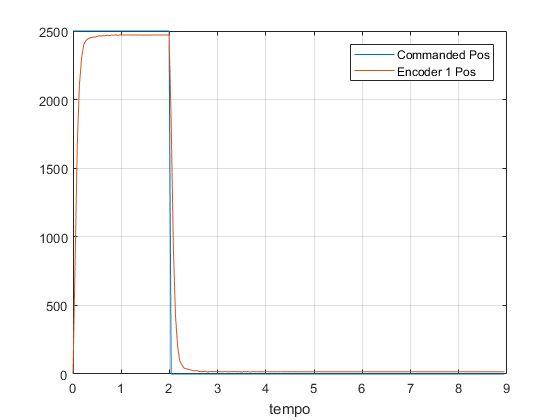
\includegraphics{q02}
\centering
\end{figure}

\pagebreak

\textbf{3.}

\begin{gather*}
    k_i k_{hw} = 7500 \implies k_i = \frac{7500}{14732} = 0.5091
\end{gather*}


\begin{figure}[H]
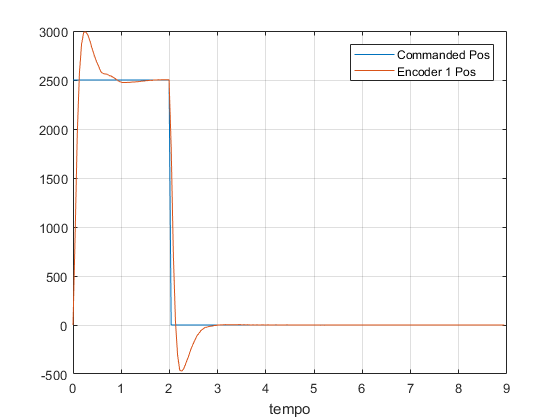
\includegraphics[scale=0.9]{q03}
\centering
\end{figure}

\textbf{4.}

\begin{figure}[H]
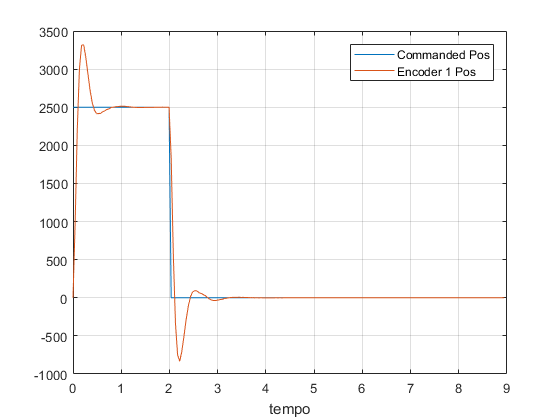
\includegraphics[scale=0.9]{q04}
\centering
\end{figure}

Como parte da força de compensação é determinada pela integral do erro; enquanto
o erro não for negativo ou zero, o termo integral aumentará de modo cumulativo.
Assim, se segurarmos o carro deslocado da origem, haverá erro e a força de
compensação irá aumentar ao longo do tempo. Se soltarmos o carro após o
segurarmos em uma posição deslocada, o carro irá acelerar em direção à posição
comandada, mas irá passar do ponto de equilíbrio e oscilar em torno dele. \\

\textbf{5.}

\begin{figure}[H]
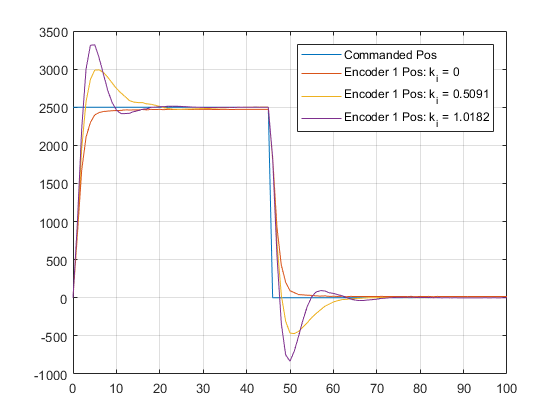
\includegraphics{q05}
\centering
\end{figure}

Como podemos ver, a ação integral elimina o erro de regime, dado que a força de
compensação aumenta enquanto houver erro. No entanto, é visível também que com
um maior ganho integral, temos um aumento visível no máximo \textit{overshoot}.
Isso pode ser explicado pelo aumento da força de compensação aplicada pelo termo
integrador, para que haja o controle ao redor do ponto de equilíbrio. Já que é
dependente do termo integrativo, essa força acumula independentemente da taxa de
variação do erro, enquanto houver erro. Com o aumento do $k_i$, há o aumento
dessa força e o sistema apresenta um \textit{overshoot} mais acentuado. \\

\pagebreak

\textbf{Procedimento experimental - parte 2}

\textbf{8.}
PI\&D, $k_i = 0$ (P\&D):

\begin{figure}[H]
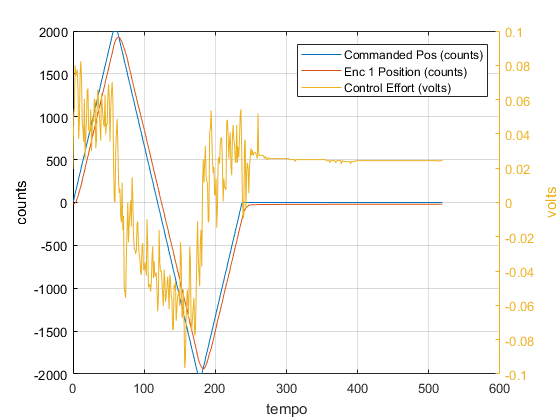
\includegraphics{q08}
\centering
\end{figure}

\textbf{9.}

PD:

\begin{figure}[H]
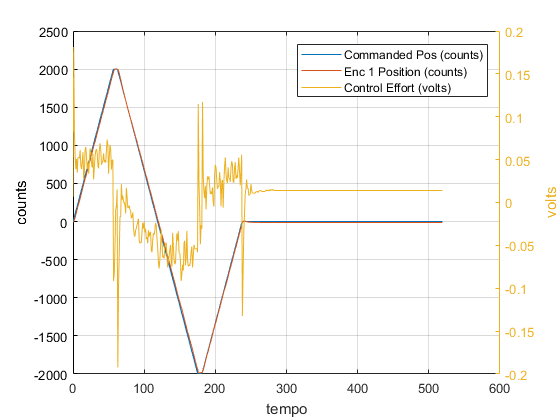
\includegraphics{q09-pd}
\centering
\end{figure}

PID:

\begin{figure}[H]
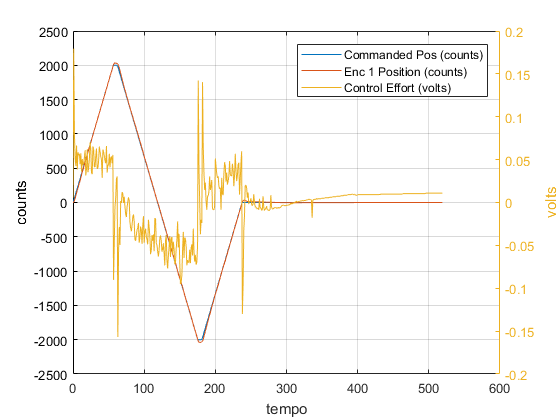
\includegraphics{q09-pid}
\centering
\end{figure}

\textbf{10.}
Para a entrada rampa, ao se usar $k_d$ no caminho direto (PID), tem-se um erro de
regime aproximadamente nulo. Ao se usar $k_d$ na realimentação (PI\&D), tem-se um
erro de regime constante. Isso justifica o que pode ser observado nos gráficos
experimentais, onde há um erro constante no sistema PI\&D, e há erro próximo de
nulo nos sistemas PD/PID.

Existe \textit{overshoot} no PID, como esperado, pois a presença do termo
integrativo adiciona \textit{overshoot} ao sistema.

Existe um \textit{control effort} bem mais acentuado no caso do P\&D do que nos
outros sistemas, pois existe um erro constante no P\&D.
Para o PD, onde o erro é próximo de nulo, o \textit{control effort} é menor
ainda, de acordo com a escala; já para o PID, o \textit{control effort} em
regime se aproxima de zero, dado seu erro mais próximo ainda de zero.

% 8-PI\&D houve erro notável, sem overshoot
% 9-PD existe erro mt mt mt pequeno. overshoot mt mt pequeno
% 9-PID houve overshoot notavel, sem erro
% TO-DO: explicar melhor essas porra

\pagebreak

\textbf{Procedimento experimental - parte 3}

\textbf{12.}

\begin{figure}[H]
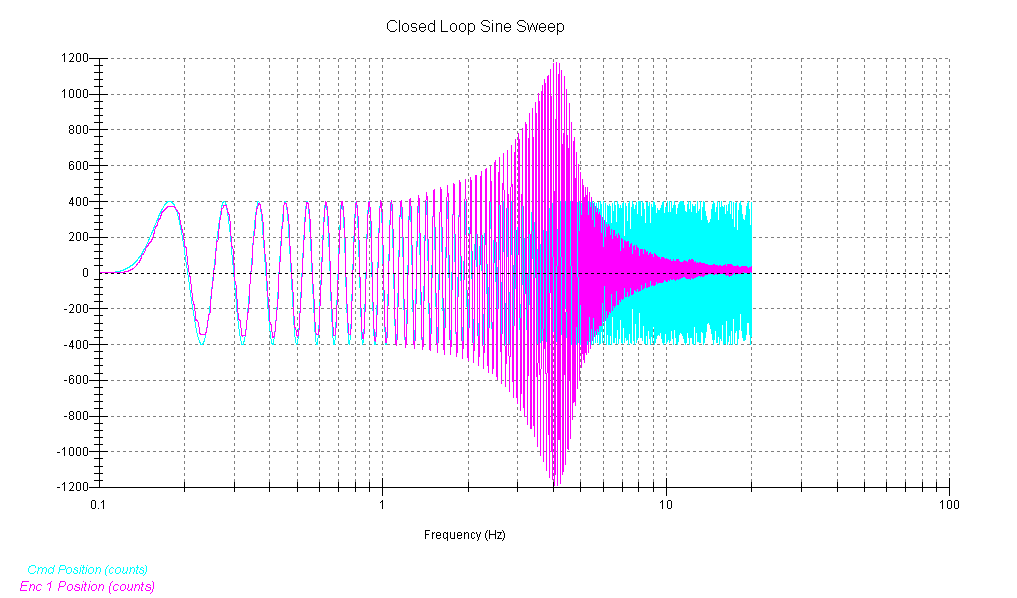
\includegraphics[scale=0.6]{q12}
\caption{Controlador P\&D}
\centering
\end{figure}

\textbf{13.}

\begin{figure}[H]
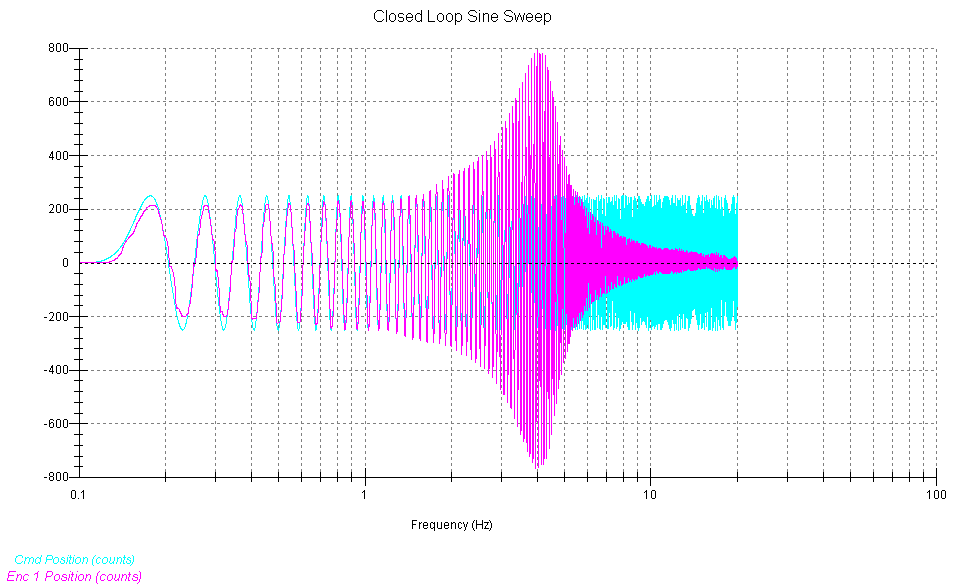
\includegraphics[scale=0.6]{q13}
\caption{Controlador PD}
\centering
\end{figure}

\textbf{14.}

% TO-DO: lembrar de fazer tanto pra PD quanto P\&D

As frequências experimentais de ressonância são de aproximadamente
$4 ~ \text{Hz}$, tanto para PD quanto P\&D.

Realizando o cálculo da frequência de ressonância teórica:

\begin{gather*}
    \omega_n := \sqrt{\frac{k_{hw} k_p}{m_1}} =
        \sqrt{\frac{14732 \cdot 0.1191}{2.778}}
        \approx 25.1316 ~ \text{(rad/s)} \\
    \xi := \frac{c_1 + k_{hw} k_d}{2 m_1 \omega_n} =
        \frac{2.94 + 14732 \cdot 0.0017}{2 \cdot 2.778 \cdot 25.1316} \approx
        0.2004 \\ \\
    \omega_r := \omega_n \sqrt{1 - 2 \xi^2} \approx 24.1010 ~ \text{(rad/s)} =
        3.9998 ~ \text{Hz}
\end{gather*}

Esse valor teórico de $3.9998 ~ \text{Hz}$ serve tanto para P\&D quanto PD, pois
as fórmulas usadas permanecem as mesmas.

Foi obtido um valor satisfatório da frequência experimental de ressonância.

% sobe 6 db/dec, desce 12 db/dec.

As curvas teóricas, com suas respectivas curvas assintóticas, são exibidas
abaixo:

\begin{figure}[H]
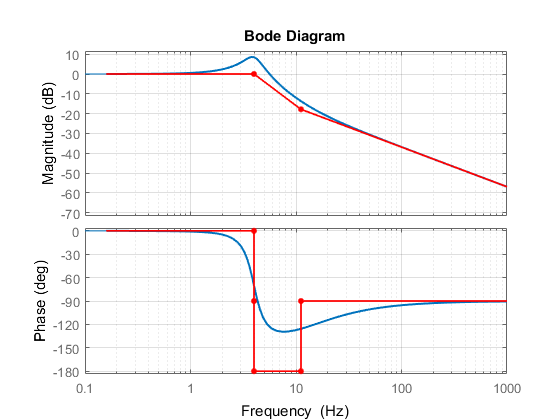
\includegraphics{q14-ped-bode-teor-assint}
\caption{Diagramas teóricos de Bode para P\&D}
\centering
\end{figure}

\begin{figure}[H]
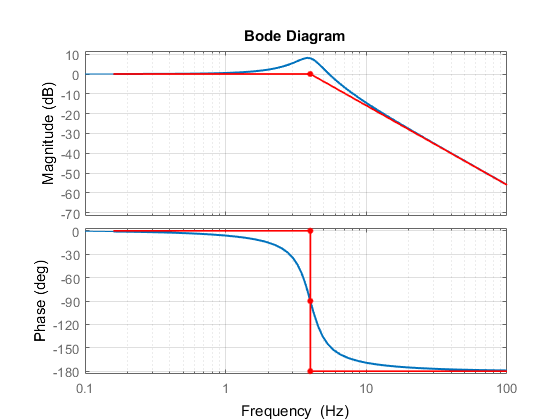
\includegraphics{q14-pd-bode-teor-assint}
\caption{Diagramas teóricos de Bode para PD}
\centering
\end{figure}

As curvas obtidas experimentalmente foram:

\begin{figure}[H]
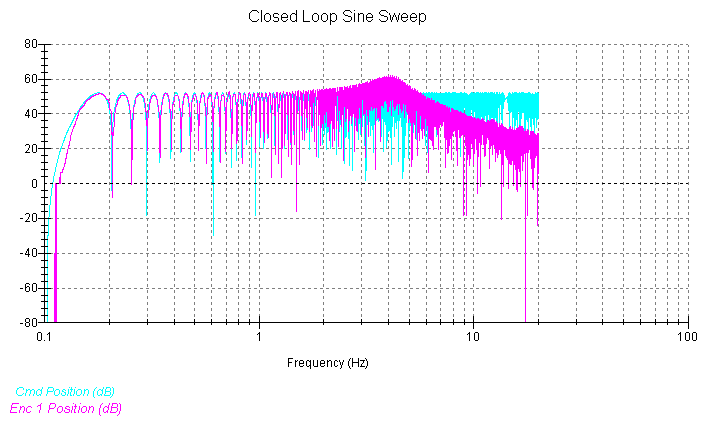
\includegraphics[scale=0.85]{q12-bode}
\caption{Gráfico experimental para P\&D}
\centering
\end{figure}

\begin{figure}[H]
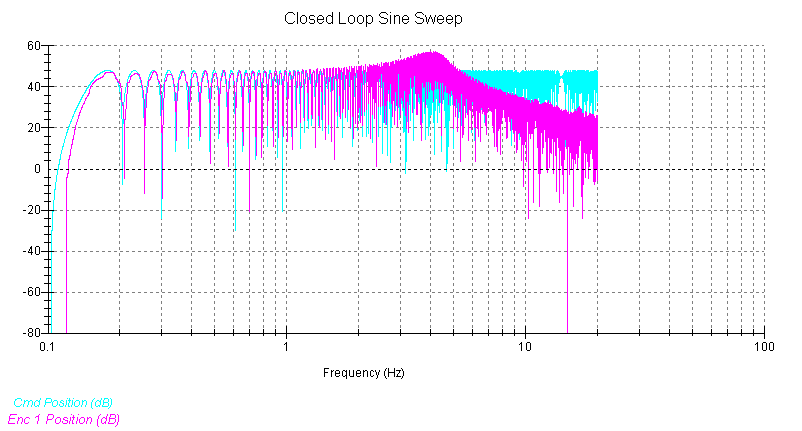
\includegraphics[scale=0.8]{q13-bode}
\caption{Gráfico experimental para PD}
\centering
\end{figure}

Os gráficos obtidos experimentalmente condizem com os gráficos teóricos
realizados.

\end{document}